% answers.tex —— 1977 年·内蒙古卷·理科 · 参考答案与详细解析片段
% 由 tools/generate_projects.py 依来源总账自 1977/1977_数学真题_内蒙古理_试题.md + 1977/1977_数学真题_内蒙古理_解析正文.md + 1977/1977_数学真题_内蒙古理_答案要点.md 生成，勿手改（改源 MD 后重跑）


\begin{gktip}
固定源是题面与解答连续出现的扫描材料。下文以第 1—6 页源解答为对照，同时重新计算关键结论；正式题为第 1—6 题，附加题保留在第 6 题解析块中。
\end{gktip}

\begin{answer}
\gksolhead{1}{}

\textbf{题目}（30 分）：

\Needspace{5\baselineskip}
（1） 化简：

\nopagebreak[4]
\[
\sqrt{4-12a+9a^2}
\]

\Needspace{5\baselineskip}
（2） 计算：

\nopagebreak[4]
\[
\frac{(-27)^3\sqrt{\left(\frac1{16}\right)^{-\frac12}}}
{(-9)^0\left(\frac32\right)^7\left(\frac12\right)^{-5}}
\]

（3） 已知 $\lg2=0.3010$，$f(x)=\log_{\sqrt{10}}x$，求 $f(5)$。

\Needspace{5\baselineskip}
（4） 求函数

\nopagebreak[4]
\[
y=\frac{\sqrt{1-\frac23x}}{\sqrt[3]{3x-1}}
\]

的定义域。

\Needspace{5\baselineskip}
（5） 已知 $\cos\theta=0.6$，$270^\circ<\theta<360^\circ$，求

\nopagebreak[4]
\[
\left(\sin\frac\theta2-\cos\frac\theta2\right)^2
\]

的值。

\Needspace{5\baselineskip}
（6） 把点 $P$ 的极坐标

\nopagebreak[4]
\[
\left(-4,-\frac{4\pi}{3}\right)
\]

化成直角坐标。

\Needspace{4\baselineskip}
\textbf{解析}

\gksubpart{（1）}

\nopagebreak[4]
\[
\sqrt{4-12a+9a^2}=\sqrt{(2-3a)^2}=\lvert2-3a\rvert
\]

\Needspace{5\baselineskip}
也可写成

\nopagebreak[4]
\[
\sqrt{4-12a+9a^2}=\begin{cases}
2-3a,&a\le\dfrac23,\\
3a-2,&a>\dfrac23
\end{cases}
\]

\gksubpart{（2）}

\nopagebreak[4]
\[
\begin{aligned}
\frac{(-27)^3\sqrt{(1/16)^{-1/2}}}
{(-9)^0(3/2)^7(1/2)^{-5}}
&=\frac{(-3)^9\sqrt4}{1\cdot3^7\cdot2^{-7}\cdot2^5}\\
&=-3^2\cdot2^3=-72
\end{aligned}
\]

\gksubpart{（3）}

\nopagebreak[4]
\[
\begin{aligned}
f(5)=\log_{\sqrt{10}}5
&=\frac{\lg5}{\lg\sqrt{10}}
=\frac{\lg10-\lg2}{\frac12\lg10}\\
&=2(1-0.3010)=1.398
\end{aligned}
\]

\gksubpart{（4）}

\Needspace{5\baselineskip}
根式要求 $1-\frac23x\ge0$，分母要求 $3x-1\ne0$，即

\nopagebreak[4]
\[
x\le\frac32,\qquad x\ne\frac13
\]

\Needspace{5\baselineskip}
故定义域为

\nopagebreak[4]
\[
(-\infty,\tfrac13)\cup(\tfrac13,\tfrac32]
\]

\gksubpart{（5）}

\Needspace{5\baselineskip}
由于 $270^\circ<\theta<360^\circ$，$\sin\theta<0$，所以

\nopagebreak[4]
\[
\sin\theta=-\sqrt{1-\cos^2\theta}=-\sqrt{1-0.6^2}=-0.8
\]

\Needspace{5\baselineskip}
从而

\nopagebreak[4]
\[
\left(\sin\frac\theta2-\cos\frac\theta2\right)^2
=1-\sin\theta=1.8
\]

\gksubpart{（6）}

\Needspace{5\baselineskip}
极坐标与直角坐标的转换式为 $x=\rho\cos\varphi$、$y=\rho\sin\varphi$。对 $\rho=-4$、$\varphi=-4\pi/3$，

\nopagebreak[4]
\[
x=-4\cos\left(-\frac{4\pi}{3}\right)=2,
\qquad
y=-4\sin\left(-\frac{4\pi}{3}\right)=-2\sqrt3
\]

所以直角坐标为 $(2,-2\sqrt3)$。

\gkanswer{答案（1）：$\lvert2-3a\rvert$。}

\gkanswer{答案（2）：$-72$。}

\gkanswer{答案（3）：$1.398$。}

\gkanswer{答案（4）：$(-\infty,\frac13)\cup(\frac13,\frac32]$。}

\gkanswer{答案（5）：$1.8$。}

\gkanswer{答案（6）：$(2,-2\sqrt3)$。}

\end{answer}
\begin{answer}
\gksolhead{2}{}

\textbf{题目}（14 分）：

（1） 已知：梯形 $ABCD$，$AD\parallel BC$，对角线 $AC$ 和 $BD$ 相交于 $E$，过 $E$ 作平行于底的直线，交 $AB$ 于 $M$，交 $CD$ 于 $N$。求证：$ME=EN$。
\nopagebreak[4]
\begin{center}% 1977 年内蒙古卷理科第 2(1) 题：梯形对角线与平行截线
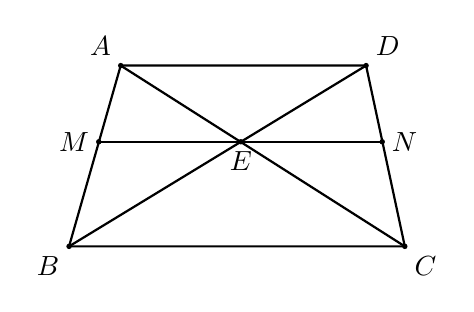
\begin{tikzpicture}[scale=0.82]
  \coordinate (A) at (0.8,2.8);
  \coordinate (D) at (4.6,2.8);
  \coordinate (B) at (0,0);
  \coordinate (C) at (5.2,0);
  \coordinate (E) at (2.66,1.62);
  \coordinate (M) at (0.46,1.62);
  \coordinate (N) at (4.85,1.62);
  \draw[thick] (A)--(D)--(C)--(B)--cycle;
  \draw[thick] (A)--(C);
  \draw[thick] (B)--(D);
  \draw[thick] (M)--(N);
  \fill (A) circle (1.2pt) node[above left] {$A$};
  \fill (D) circle (1.2pt) node[above right] {$D$};
  \fill (B) circle (1.2pt) node[below left] {$B$};
  \fill (C) circle (1.2pt) node[below right] {$C$};
  \fill (E) circle (1.2pt) node[below] {$E$};
  \fill (M) circle (1.2pt) node[left] {$M$};
  \fill (N) circle (1.2pt) node[right] {$N$};
\end{tikzpicture}
\end{center}
\nopagebreak[4]
（2） 圆台上底直径为 $12\ \mathrm{cm}$，下底直径为 $24\ \mathrm{cm}$，高为 $8\ \mathrm{cm}$，求圆台的全面积。（$\pi\approx3.14$，精确到 $0.1\ \mathrm{cm^2}$。）

\Needspace{4\baselineskip}
\textbf{解析}

\gksubpart{（1）}

\Needspace{5\baselineskip}
由 $AD\parallel MN\parallel BC$ 以及对角线交点的相似三角形关系，

\nopagebreak[4]
\[
\frac{AM}{AB}=\frac{DN}{DC}
\]

\Needspace{5\baselineskip}
又由 $\triangle EAM\sim\triangle ECB$、$\triangle EDN\sim\triangle EBC$，得到

\nopagebreak[4]
\[
\frac{ME}{BC}=\frac{AM}{AB},
\qquad
\frac{EN}{BC}=\frac{DN}{DC}
\]

\Needspace{5\baselineskip}
因此 $ME/BC=EN/BC$，从而

\nopagebreak[4]
\[
ME=EN
\]

\gksubpart{（2）}

\Needspace{5\baselineskip}
上、下底半径分别为

\nopagebreak[4]
\[
r_1=\frac{12}{2}=6\ \mathrm{cm},
\qquad
r_2=\frac{24}{2}=12\ \mathrm{cm},
\qquad h=8\ \mathrm{cm}
\]

\Needspace{5\baselineskip}
圆台母线长为

\nopagebreak[4]
\[
l=\sqrt{h^2+(r_2-r_1)^2}=\sqrt{8^2+6^2}=10\ \mathrm{cm}
\]

\Needspace{5\baselineskip}
全面积为

\nopagebreak[4]
\[
\begin{aligned}
S&=\pi\bigl[r_1^2+r_2^2+(r_1+r_2)l\bigr]\\
&=3.14(36+144+18\times10)\\
&=1130.4\ \mathrm{cm^2}
\end{aligned}
\]

\gkanswer{答案（1）：$ME=EN$，证明见解析版。}

\gkanswer{答案（2）：$1130.4\ \mathrm{cm^2}$。}

\end{answer}
\begin{answer}
\gksolhead{3}{}

\textbf{题目}（12 分）：

红旗拖拉机厂今年元月份生产出一批甲、乙两种型号的拖拉机，其中生产乙型 16 台。从二月份起，甲型每月增产 10 台，而乙型按每月相同增长率逐步递增。又知二月份甲、乙两型拖拉机产量之比是 $3:2$，三月份甲、乙两型拖拉机产量之和是 65 台。求乙型拖拉机每月的增长率及甲型拖拉机元月份的产量。

\Needspace{4\baselineskip}
\textbf{解析}

\Needspace{5\baselineskip}
设乙型拖拉机每月增长率为 $x$，甲型拖拉机元月份产量为 $y$ 台。由二月份产量比和三月份总量得

\nopagebreak[4]
\[
\frac{y+10}{16(1+x)}=\frac32,
\qquad
y+20+16(1+x)^2=65
\]

\Needspace{5\baselineskip}
第一式给出 $y=24x+14$。代入第二式：

\nopagebreak[4]
\[
16x^2+56x-15=0
\quad\Longleftrightarrow\quad
(4x-1)(4x+15)=0
\]

\Needspace{5\baselineskip}
增长率取非负的合理值，故 $x=1/4=25\%$，并有

\nopagebreak[4]
\[
y=24\times\frac14+14=20
\]

\gkanswer{答案：乙型拖拉机每月增长率为 $25\%$，甲型拖拉机元月份产量为 $20$ 台。}

\end{answer}
\begin{answer}
\gksolhead{4}{}

\textbf{题目}（14 分）：

已知：直线 $3x+y=5$ 及 $2x-3y+4=0$ 交于 $A$ 点。求：

（1） 过 $A$ 点且与 $y$ 轴垂直的直线方程；

（2） 过 $A$ 点且与圆 $x^2+y^2=1$ 相切的直线方程。

\Needspace{4\baselineskip}
\textbf{解析}

\Needspace{5\baselineskip}
联立两条已知直线：

\nopagebreak[4]
\[
\begin{cases}
3x+y=5,\\
2x-3y+4=0
\end{cases}
\quad\Longrightarrow\quad A=(1,2)
\]

\gksubpart{（1）}

\Needspace{5\baselineskip}
与 $y$ 轴垂直的直线为水平线，所以方程为

\nopagebreak[4]
\[
y=2
\]

\gksubpart{（2）}

\Needspace{5\baselineskip}
设圆 $x^2+y^2=1$ 的切点为 $P=(u,v)$。过 $A=(1,2)$ 的切线共有两条：一条为过 $(1,0)$ 的竖直线 $x=1$，另一条经验证为

\nopagebreak[4]
\[
3x-4y+5=0
\]

该直线到原点的距离为 $5/5=1$，故确为单位圆切线。

\gkanswer{答案（1）：$y=2$。}

\gkanswer{答案（2）：$3x-4y+5=0$ 或 $x=1$。}

\end{answer}
\begin{answer}
\gksolhead{5}{}

\textbf{题目}（15 分）：

甲、乙两船，甲船在某岛 $B$ 的正南方向 $A$ 处，$AB=10$ 海里，甲船自 $A$ 处以 $4$ 海里/小时的速度向正北方向航行；同时，乙船以 $6$ 海里/小时的速度自 $B$ 出发，向岛的北 $60^\circ$ 西方向驶去，问几分钟后两船相距最近？（精确到 1 分。）
\nopagebreak[4]
\begin{center}% 1977 年内蒙古卷理科第 5 题：两船航行示意图
\begin{tikzpicture}[scale=0.68]
  \coordinate (A) at (0,0);
  \coordinate (B) at (0,5.0);
  \coordinate (C) at (0,2.25);
  \coordinate (D) at (2.8,5.0);
  \draw[thick] (A)--(B);
  \draw[thick] (B)--(D);
  \draw[thick] (C)--(D);
  \draw[dashed] (C)--(B);
  \fill (A) circle (1.2pt) node[below left] {$A$};
  \fill (B) circle (1.2pt) node[left] {$B$};
  \fill (C) circle (1.2pt) node[left] {$C$};
  \fill (D) circle (1.2pt) node[right] {$D$};
  \node[right] at (0,3.65) {甲船};
  \node[above] at (1.35,5.0) {乙船};
  \node[right] at (0,2.25) {$4x$};
  \node[left] at (0,3.6) {$10-4x$};
  \node[above] at (1.4,5.0) {$6x$};
  \node at (1.0,4.1) {$60^\circ$};
\end{tikzpicture}
\end{center}
\nopagebreak[4]
\Needspace{4\baselineskip}
\textbf{解析}

\Needspace{5\baselineskip}
设经过 $x$ 小时后，甲船到达 $C$，乙船到达 $D$。则

\nopagebreak[4]
\[
AC=4x,\qquad BC=10-4x,\qquad BD=6x
\]

\Needspace{5\baselineskip}
在三角形 $BCD$ 中，$\angle DBC=180^\circ-60^\circ=120^\circ$。由余弦定理，

\nopagebreak[4]
\[
\begin{aligned}
DC^2&=(6x)^2+(10-4x)^2-2\cdot6x(10-4x)\cos120^\circ\\
&=28x^2-20x+100\\
&=28\left(x-\frac5{14}\right)^2+\frac{675}{7}
\end{aligned}
\]

所以当 $x=5/14$ 小时时距离最小，即约 $21$ 分钟后两船相距最近。

\gkanswer{答案：约 $21$ 分钟后两船相距最近。}

\end{answer}
\begin{answer}
\gksolhead{6}{}

\textbf{题目}（15 分）：

已知：在 $\triangle ABC$ 中，$a\text{、}b\text{、}c$ 是三个内角 $A\text{、}B\text{、}C$ 的对边，$\lg\sin A\text{、}\lg\sin B\text{、}\lg\sin C$ 成等差数列。

\Needspace{5\baselineskip}
（1） 求证：

\nopagebreak[4]
\[
\frac{\sin^2A}{\sin^2B}=\frac ac
\]

\Needspace{5\baselineskip}
（2） 又若方程

\nopagebreak[4]
\[
cx^2+2cx+a=0
\]

有相等的两个实根，求证：$\sin A=\sin B=\sin C$。

\begin{gktip}
\textbf{附加题（20 分，不计入总分）}
\end{gktip}

\Needspace{5\baselineskip}
\textbf{附加题 1．} 在 $\triangle ABC$ 中，求证：

\nopagebreak[4]
\[
\sin^2A+\sin^2B+\cos^2C+2\sin A\sin B\cos(A+B)=1
\]

\Needspace{5\baselineskip}
\textbf{附加题 2．} 已知：椭圆的中心点在原点，长轴和短轴都在坐标轴上，离心率 $e=0.8$，一条准线方程为

\nopagebreak[4]
\[
y=-\frac{25}{4}
\]

求内接于椭圆的最大矩形面积。

\Needspace{4\baselineskip}
\textbf{解析}

\gksubpart{（1）}

\Needspace{5\baselineskip}
由于 $\lg\sin A$、$\lg\sin B$、$\lg\sin C$ 成等差数列，

\nopagebreak[4]
\[
2\lg\sin B=\lg\sin A+\lg\sin C
\]

\Needspace{5\baselineskip}
即

\nopagebreak[4]
\[
\sin^2B=\sin A\sin C
\]

\Needspace{5\baselineskip}
由正弦定理 $\sin C/\sin A=c/a$，所以

\nopagebreak[4]
\[
\sin^2B=\frac ca\sin^2A
\quad\Longrightarrow\quad
\frac{\sin^2A}{\sin^2B}=\frac ac
\]

\gksubpart{（2）}

\Needspace{5\baselineskip}
方程 $cx^2+2cx+a=0$ 有相等的两个实根，因此

\nopagebreak[4]
\[
(2c)^2-4ca=4c(c-a)=0
\]

\Needspace{5\baselineskip}
三角形边长 $c>0$，故 $a=c$，从而 $A=C$。结合（1）式有 $\sin^2A=\sin^2B$。三角形内角均在 $0^\circ$ 与 $180^\circ$ 之间，且 $A=C$，排除退化情形后得 $A=B=C=60^\circ$，所以

\nopagebreak[4]
\[
\sin A=\sin B=\sin C
\]

\gksubpart{附加题 1}

\Needspace{4\baselineskip}
\textbf{解析}

\Needspace{5\baselineskip}
由 $A+B+C=180^\circ$，有 $\cos C=-\cos(A+B)$。于是

\nopagebreak[4]
\[
\begin{aligned}
&\sin^2A+\sin^2B+\cos^2C+2\sin A\sin B\cos(A+B)\\
&=\sin^2A+\sin^2B+\cos^2(A+B)+2\sin A\sin B\cos(A+B)\\
&=\sin^2A+\sin^2B+\bigl(\cos A\cos B-\sin A\sin B\bigr)^2\\
&\quad+2\sin A\sin B\bigl(\cos A\cos B-\sin A\sin B\bigr)\\
&=\cos^2B(\sin^2A+\cos^2A)+\sin^2B\\
&=1
\end{aligned}
\]

\gksubpart{附加题 2}

\Needspace{4\baselineskip}
\textbf{解析}

\Needspace{5\baselineskip}
设椭圆长半轴为 $a$，短半轴为 $b$，半焦距为 $c$。离心率为 $e=c/a=0.8$，且竖直方向为长轴方向时，一条准线为 $y=-a/e$。由题给准线

\nopagebreak[4]
\[
\frac{a}{0.8}=\frac{25}{4}
\quad\Longrightarrow\quad
a=5,\qquad c=4
\]

\Needspace{5\baselineskip}
再由 $b^2=a^2-c^2$ 得 $b=3$，椭圆方程为

\nopagebreak[4]
\[
\frac{x^2}{3^2}+\frac{y^2}{5^2}=1
\]

\Needspace{5\baselineskip}
将椭圆沿坐标轴方向缩放回单位圆后，内接矩形的最大面积对应于圆内接正方形。因此原椭圆内接最大矩形的面积为

\nopagebreak[4]
\[
2ab=2\times3\times5=30
\]

\gkanswer{答案（1）：见解析版。}

\gkanswer{答案（2）：$\sin A=\sin B=\sin C$。}

\end{answer}